\documentclass[12pt]{article}

%\usepackage{fullpage}
%\usepackage{epic}
%\usepackage{eepic}
%\usepackage{graphicx}

\usepackage{listings} % Code
\usepackage{fancyhdr} % header footer
\usepackage{xcolor}  % Color
\usepackage{mathtools} % Math

\usepackage{geometry}
 \geometry{
 a4paper,
 total={170mm,257mm},
 left=20mm,
 top=20mm,
 }

%\newcommand{\proof}[1]{
%{\noindent {\it Proof.} {#1} \rule{2mm}{2mm} \vskip \belowdisplayskip}
%}


%\newtheorem{lemma}{Lemma}[section]
%\newtheorem{theorem}[lemma]{Theorem}
%\newtheorem{claim}[lemma]{Claim}
%\newtheorem{definition}[lemma]{Definition}
%\newtheorem{corollary}[lemma]{Corollary}

%\setlength{\oddsidemargin}{0in}
%\setlength{\topmargin}{0in}
%\setlength{\textwidth}{6.5in}
%\setlength{\textheight}{8.5in}

\cfoot{footer}

\lstset {
%language=Java,
backgroundcolor = \color{lightgray},
                   language = Java,
                   xleftmargin = 2mm,
                   framexleftmargin = 1em
%lineskip={-1.5pt}
}

%\usepackage[utf8]{inputenc}
 
 
% Information about contents section
\title{Contents}
\author{Rudra Nil Basu}
\date{ }
 
\renewcommand*\contentsname{Summary}

\begin{document}

% to generate the contents page
\maketitle
\tableofcontents

\newpage

\setlength{\fboxrule}{.5mm}\setlength{\fboxsep}{1.2mm}
\newlength{\boxlength}\setlength{\boxlength}{\textwidth}
\addtolength{\boxlength}{-4mm}
\begin{center}\framebox{\parbox{\boxlength}{\bf
CS594D: Object Oriented Programming \hfill 
Date: 11/10/2016
\\
%DATE
\hfill
}}\end{center}
\vspace{5mm}

\section{Week 1 - Operation with numbers and patterns}

%The text of the notes goes here.
%To include a theorem with proof, use the following format.

\textbf{Problem 1.1} \textit{Write a program in Java to find the prime numbers between 1 to 100}\\


\textit{Code.}



\begin{lstlisting}[language=Java]
class prime
{
	static boolean primes[];
	public static void fillFalse()
	{
		int i;
		for(i=0;i<101;i++) {
			primes[i]=true;
		}
	}
	public static void initialise()
	{
		fillFalse();
		int i,j;
		primes[1]=false;
		for(i=2;i<101;i++) {
			if(primes[i]==true) {
				for(j=i+i;j<101;j+=i) {
					primes[j]=false;
				}
			}
		}
	}
	public static void print()
	{
		int i;
		for(i=1;i<=100;i++) {
			if(primes[i]==true)
			System.out.print(i+" ");
		}
	}
	public static void main(String ags[])
	{
		primes=new boolean[101];
		initialise();
		print();
	}
}
\end{lstlisting}

\textit{Output.}
\begin{lstlisting}
2 3 5 7 11 13 17 19 23 29 31 37 41 43 47 53 59 61 67 71 73 79 83 89 
97 
\end{lstlisting}

\textbf{Problem 1.2} \textit{Write a program in Java to reverse a given number.}\\


\textit{Code.}

\begin{lstlisting}[language=Java]
import java.io.*;
class reverse
{
	public static void main(String args[])throws IOException
	{
		BufferedReader br=new BufferedReader(new 
		InputStreamReader(System.in));
		int n;
		n=Integer.parseInt(br.readLine());
		int m=n,rev=0;
		while(m>0) {
			rev=(rev*10)+m%10;
			m/=10;
		}
		System.out.println("Reversed Number "+rev);
	}
}
\end{lstlisting}

\textit{Output.}
\begin{lstlisting}
12345
Reversed Number 54321
\end{lstlisting}

\textbf{Problem 1.3} \textit{Write a program in Java to find the sum of digits of a given number.}\\


\textit{Code.}

\begin{lstlisting}[language=Java]
import java.io.*;
class sum
{
	public static void main(String args[])throws IOException
	{
		BufferedReader br=new BufferedReader(new 
		InputStreamReader(System.in));
		int n;
		n=Integer.parseInt(br.readLine());
		int m=n,rev=0,sum=0;
		while(m>0) {
			sum+=(m%10);
			m/=10;
		}
		System.out.println("Sum of each digits "+sum);
	}
}
\end{lstlisting}

\textit{Output.}
\begin{lstlisting}
12345
Sum of each digits 15
\end{lstlisting}

\textbf{Problem 1.4} \textit{Write a program in Java to print the following pattern.}

\begin{lstlisting}
*
**
***
****
\end{lstlisting}

\textit{Code.}

\begin{lstlisting}[language=Java]
class patt1
{
	public static void main(String args[])
	{
		int n=4,i,j;
		for(i=1;i<=n;i++) {
			for(j=1;j<=i;j++) {
				System.out.print("*");
			}
			System.out.println();
		}
	}
}
\end{lstlisting}

\textit{Output.}
\begin{lstlisting}
*
**
***
****
\end{lstlisting}

\textbf{Problem 1.5} \textit{Write a program in Java to print the following pattern.}

\begin{lstlisting}
   *
  ***
 *****
*******
\end{lstlisting}

\textit{Code.}

\begin{lstlisting}[language=Java]
class patt2
{
	public static void main(String args[])
	{
		int n=4,i,j,k;
		for(i=1;i<=n;i++) {
			for(j=n-1;j>=i;j--) {
				System.out.print(" ");
			}
			for(j=1;j<=((2*i)-1);j++) {
				System.out.print("*");
			}
			System.out.println();
		}
	}
}
\end{lstlisting}

\textit{Output.}
\begin{lstlisting}
   *
  ***
 *****
*******
\end{lstlisting}

\textbf{Problem 1.6} \textit{Write a program in Java to print the following pattern.}

\begin{lstlisting}
   *
  **
 ***
****
\end{lstlisting}

\textit{Code.}

\begin{lstlisting}[language=Java]
class patt3
{
	public static void main(String args[])
	{
		int n=4,i,j;
		for(i=1;i<=n;i++) {
			for(j=n-1;j>=i;j--) {
				System.out.print(" ");
			}
			for(j=1;j<=i;j++) {
				System.out.print("*");
			}
			System.out.println();
		}
	}
}
\end{lstlisting}

\textit{Output.}
\begin{lstlisting}
   *
  **
 ***
****
\end{lstlisting}

\newpage

% Week 2

\setlength{\fboxrule}{.5mm}\setlength{\fboxsep}{1.2mm}
%\newlength{\boxlength}\setlength{\boxlength}{\textwidth}
\addtolength{\boxlength}{-4mm}
\begin{center}\framebox{\parbox{\boxlength}{\bf
CS594D: Object Oriented Programming \hfill 
Date: 18/10/2016
\\
%DATE
\hfill
}}\end{center}
\vspace{5mm}

\section{Week 2 - Function and Constructor Overloading}

%Function and Constructor Overloading

\textbf{Problem 2.1} \textit{Write a program in Java to calculate the area of different shapes using function overloading.}


\textit{Code.}

\begin{lstlisting}[language=Java]
class area1
{
	void area(int sq)
	{
		System.out.println("Area of Square = "+sq*sq);
	}
	void area(int l, int w)
	{
		System.out.println("Area of Rectangle = "+l*w);
	}
	void area(float b,float ht)
	{
		System.out.println("Area of Triangle = "+(0.5)*(b*ht));
	}
	public static void main(String args[])
	{
		area1 a1=new area1();
		a1.area(10);
		a1.area(10,20);
		a1.area(10.0f,25.0f);
	}
}
\end{lstlisting}

\textit{Output.}
\begin{lstlisting}
Area of Square = 100
Area of Rectangle = 200
Area of Triangle = 125.0
\end{lstlisting}



\textbf{Problem 2.1} \textit{Write a program in Java to calculate the area of different shapes using Constructor overloading.}


\textit{Code.}

\begin{lstlisting}[language=Java]
class area2
{
	area2(int sq)
	{
		System.out.println("Area of Square = "+sq*sq);
	}
	area2(int l, int w)
	{
		System.out.println("Area of Rectangle = "+l*w);
	}
	area2(float b,float ht)
	{
		System.out.println("Area of Triangle = "+(0.5)*(b*ht));
	}
	public static void main(String args[])
	{
		area2 a1=new area2(5);
		a1=new area2(12,20);
		a1=new area2(12.5f,13.0f);
	}
}
\end{lstlisting}

\textit{Output.}
\begin{lstlisting}
Area of Square = 25
Area of Rectangle = 240
Area of Triangle = 81.25
\end{lstlisting}

\newpage

\setlength{\fboxrule}{.5mm}\setlength{\fboxsep}{1.2mm}
%\newlength{\boxlength}\setlength{\boxlength}{\textwidth}
\addtolength{\boxlength}{-4mm}
\begin{center}\framebox{\parbox{\boxlength}{\bf
CS594D: Object Oriented Programming \hfill 
Date: 1/11/2016
\\
%DATE
\hfill
}}\end{center}
\vspace{5mm}

\section{Week 3 - Objects}

\textbf{Problem 3.1} \textit{Write a program to design a class representing a bank account. The class should have the following data members:\\
* a/c no. * customer id * balance amount\\
The class should have member methods with the following functions:\\
* initialize initial value
* to deposit amount
* to withdraw amount
* to display customer id, a/c no. and current balance.}


\textit{Code.}

\begin{lstlisting}[language=Java]
import java.util.*;
class Bank{
	static Scanner sc=new Scanner(System.in);
	static long acno; static double amt;
	static String id;
	private void init(){
		acno=0; amt=0.0;
		id="";
	}
	private double deposit(double d){ return amt+=d; }
	private double withdraw(double d){
		if(d<amt&&amt!=0)return amt-=d;
		else {
			 System.out.println("Not Enough Balance!!");
			  return amt;
		}
	}
	private void print(){
		System.out.println("Customer ID \t A/c No. \t"+
		"Current Balance");
		System.out.println(id+"\t \t "+acno+"\t \t "+amt);
	}
	public static void main(String[]args){
		Bank obj=new Bank();
		obj.init();
		System.out.println("Enter account no and current balance:");
		id="3000114022";
		acno=sc.nextLong(); amt=sc.nextDouble();
		double d=0.0;
		int choice=0;
		do{
			System.out.println("Main Menu");
			System.out.println("0. Deposit");
			System.out.println("1. Withdrawal");
			System.out.println("2. Print Statement");
			System.out.println("3. Exit");
			System.out.println("Enter choice:");
			choice=sc.nextInt();
			switch(choice){
				case 0:d=0.0;
				        System.out.println("Enter "+
				        "amount to deposit:");
				        d=sc.nextDouble();
					 System.out.println("Deposit="+d+
					 "current balance="+
					 (double)obj.deposit(d));
					 break;
				case 1:d=0.0;
				       System.out.println("Amount ?");
				       d=sc.nextDouble();
				       System.out.println("withdrawal="+d+
				       "current balance="+
				       (double)obj.withdraw(d));
				        break;
				case 2:obj.print();
				       break;
				default:
					break;
			}
		}while(choice<3);
	}
}

\end{lstlisting}

\textit{Output.}
\begin{lstlisting}
Enter account no and current balance:
1200
10000
Main Menu
0. Deposit
1. Withdrawal
2. Print Statement
3. Exit
Enter choice
0
Enter amount to deposit
2000
Deposit=2000.0 current balance=12000.0
Main Menu
0. Deposit
1. Withdrawal
2. Print Statement
3. Exit
Enter choice
1
Amount ?
3000
withdrawal = 3000.0 current balance=9000.0
Main Menu
0. Deposit
1. Withdrawal
2. Print Statement
3. Exit
Enter choice
1
Amount?
15000
Not Enough Balance!!
\end{lstlisting}

\textbf{Problem 3.2} \textit{Write a program to add two complex numbers.\\
Print the result in \(x+iy\)\\
form. Use objects as arguments to a method which will perform the addition
and use function overloading.}


\textit{Code.}

\begin{lstlisting}
class Complex
{
	double x;
	int y;
	Complex(double a,int b){
		x=a; y=b;
	}
	void print(){ System.out.println(x+"+ i"+y); }
}
class Test{
	double real; int imag;
	private double sum(double a,double b){
		real=a+b; return real;
	}
	private int sum(int a,int b){
		imag=a+b; return imag;
	}
	public static void main(String[]args){
		Complex obj=new Complex(4,6);
		obj.print();
		Complex obj1=new Complex(1,9);
		obj1.print();
		Test t1=new Test();
		System.out.println("sum =: "+t1.sum(obj.x,obj1.x)+"+i"
		+t1.sum(obj.y,obj1.y));
	}
}

\end{lstlisting}

\textit{Output.}

\begin{lstlisting}
4.0+ i6
1.0+ i9
sum =: 5.0+i15
\end{lstlisting}

\newpage

\setlength{\fboxrule}{.5mm}\setlength{\fboxsep}{1.2mm}
%\newlength{\boxlength}\setlength{\boxlength}{\textwidth}
\addtolength{\boxlength}{-4mm}
\begin{center}\framebox{\parbox{\boxlength}{\bf
CS594D: Object Oriented Programming \hfill 
Date: 8/11/2016
\\
%DATE
\hfill
}}\end{center}
\vspace{5mm}

\section{Week 4 - Command Line Arguments \& static variables}

\textbf{Problem 4.2} \textit{Write a program in Java and create a Student classes such that all the students have unique roll no}

\textit{Code.}
\begin{lstlisting}
class Student
{
	static int count;
	int roll;
	Student()
	{
		roll=++count;
	}
	int showRoll()
	{
	    return roll;
	}
}
class st
{
	public static void main(String args[])
	{
		Student a=new Student();
		Student b=new Student();
		Student c=new Student();
		System.out.println("Roll of Student A = "+a.showRoll());
		System.out.println("Roll of Student B = "+b.showRoll());
		System.out.println("Roll of Student C = "+c.showRoll());
	}
}
\end{lstlisting}

\textit{Output.}
\begin{lstlisting}
Roll of Student A = 1
Roll of Student B = 2
Roll of Student C = 3
\end{lstlisting}

\textbf{Problem 4.2} \textit{Write a program in Java and create two sub classes "Arts" and "Science", such that all the students have unique roll no}


\textit{Code.}

\begin{lstlisting}[language=Java]
class Student
{
	static int count;
	int roll;
	Student()
	{
		roll=++count;
	}
}
class Science extends Student
{
	int phy,chem,math;
	Science(int _phy, int _chem, int _math)
	{
		super();
		phy=_phy;
		chem=_chem;
		math=_math;
	}
}
class Art extends Student
{
	int hist,geo,eng;
	Art(int _hist, int _geo, int _eng)
	{
		super();
		hist=_hist;
		geo=_geo;
		eng=_eng;
	}
}
class st
{
	public static void main(String args[])
	{
		Art a1=new Art(10,20,30);
		Science s1=new Science(15,25,31);
		System.out.println("Art\t\t"+a1.hist+
		"\t"+a1.geo+"\t"+a1.eng+"\tRoll "+a1.roll);
		System.out.println("Science\t\t"+s1.phy+"\t"+s1.chem+
		"\t"+s1.math+"\tRoll "+s1.roll);
	}
}
\end{lstlisting}
\textit{Output.}

\begin{lstlisting}
Art		10	20	30	Roll 1
Science		15	25	31	Roll 2
\end{lstlisting}

\textbf{Problem 4.3} \textit{Write a program in Java to take two integers from the command line and print the largest and smallest among them.}


\textit{Code.}

\begin{lstlisting}
class op
{
	public static void main(String args[])
	{
		int i;
		int a=Integer.parseInt(args[0]);
		int b=Integer.parseInt(args[1]);
		System.out.println("Sum="+(a+b));
		int max,min;
		if(a>b) {
			max=a;
			min=b;
		} else {
			max=b;
			min=a;
		}
		System.out.println("Max="+max+"\nMin="+min);

	}
}
\end{lstlisting}
\textit{Output.}

\begin{lstlisting}
Max=5
Min=-1
\end{lstlisting}

\textbf{Problem 4.4} \textit{Write a program in Java to take command line integers from argument and sort them.}


\textit{Code.}

\begin{lstlisting}
class sot
{
	public static void main(String args[])
	{
		int i,j;
		int n=args.length;
		int a[]=new int[n];
		for(i=0;i<n;i++) {
			a[i]=Integer.parseInt(args[i]);
		}
		for(i=0;i<n-1;i++) {
			for(j=0;j<n-i-1;j++) {
				if(a[j]>a[j+1]) {
					a[j]=(a[j]+a[j+1])-(a[j+1]=a[j]);
				}
			}
		}
		for(i=0;i<n;i++) {
			System.out.println(a[i]);
		}
	}
}
\end{lstlisting}
\textit{Output.}

\begin{lstlisting}
1
3
5
7
\end{lstlisting}

\textbf{Problem 4.5} \textit{Write a program in Java to take command line float from argument and sort them.}


\textit{Code.}

\begin{lstlisting}
class sortF
{
	public static void main(String args[])
	{
		int i,j;
		int n=args.length;
		float a[]=new float[n];
		for(i=0;i<n;i++) {
			a[i]=Float.parseFloat(args[i]);
		}
		for(i=0;i<n-1;i++) {
			for(j=0;j<n-i-1;j++) {
				if(a[j]>a[j+1]) {
					a[j]=(a[j]+a[j+1])-
					(a[j+1]=a[j]);
				}
			}
		}
		for(i=0;i<n;i++) {
			System.out.println(a[i]);
		}
	}
}
\end{lstlisting}
\textit{Output.}

\begin{lstlisting}
1.5
2.1
2.5
3.4
5.0
\end{lstlisting}

\textbf{Problem 4.6} \textit{Write a program in Java to take command line strings from argument and sort them.}


\textit{Code.}

\begin{lstlisting}
class sortAR
{
	public static void main(String args[])
	{
		int i,j;
		for(i=0;i<args.length-1;i++) {
			for(j=0;j<args.length-i-1;j++) {
				if(args[j].compareTo(args[j+1])>0) {
					String temp=args[j+1];
					args[j+1]=args[j];
					args[j]=temp;
				}
			}
		}
		for(i=0;i<args.length;i++) {
			System.out.println(args[i]);
		}
	}
}
\end{lstlisting}
\textit{Output.}

\begin{lstlisting}
Debayan
Rohit
Rudra
\end{lstlisting}

\newpage

\setlength{\fboxrule}{.5mm}\setlength{\fboxsep}{1.2mm}
%\newlength{\boxlength}\setlength{\boxlength}{\textwidth}
\addtolength{\boxlength}{-4mm}
\begin{center}\framebox{\parbox{\boxlength}{\bf
CS594D: Object Oriented Programming \hfill 
Date: 15/11/2016
\\
%DATE
\hfill
}}\end{center}
\vspace{5mm}

\section{Week 5 - Sorting of Objects}

\textbf{Problem 5.1} \textit{Write a program in Java to create a Student class and arrange the objects according to their percentage}


\textit{Code.}

\begin{lstlisting}
class Student
{
	String name;
	float per;
	void init(String _name, float _per)
	{
		name=_name;
		per=_per;
	}
	public static void main(String args[])
	{
		Student s[]=new Student[3];
		int i,j;
		for(i=0;i<3;i++) {
			s[i]=new Student();
		}
		s[0].name="Rudra";s[0].per=50.0f;
		s[1].name="Tokon";s[1].per=99.99f;
		s[2].name="Rohit";s[2].per=98.99f;
		for(i=0;i<3-1;i++) {
			for(j=0;j<3-i-1;j++) {
				if(s[i].per>s[i+1].per) {
					Student temp=s[i];
					s[i]=s[i+1];
					s[i+1]=temp;
				}
			}
		}
		for(i=0;i<3;i++) {
			System.out.println("Name="+s[i].name+
			" Percentage="+s[i].per);
		}
	}
}
\end{lstlisting}
\textit{Output.}
\begin{lstlisting}
Name=Rudra Percentage=50.0
Name=Rohit Percentage=98.99
Name=Tokon Percentage=99.99
\end{lstlisting}

\textbf{Problem 5.2} \textit{Write a program in Java using vectors to do the following program. Create objects of 2 classes "Arts" and "Science". Depending on the argument, retrieve the objects, sort the objects according to their marks and display them. Try to use all concepts of Java so far.}


\textit{Code.}

\begin{lstlisting}
import java.io.*;

class Student
{
	String name;
	int roll;
	int marks1;
	int marks2;
	int marks3;
	float perc;
	void init(String _name, int _roll,
	 int _marks1, int _marks2, int _marks3)
	{
		name=_name;
		roll=_roll;
		marks1=_marks1;
		marks2=_marks2;
		marks3=_marks3;
	}
	void calcPerc()
	{
		perc=(marks1+marks2+marks3)/3.0f;
	}
}

class StDetails
{
	public static void main(String args[]) throws IOException
	{
		BufferedReader br= new BufferedReader(new 
		InputStreamReader(System.in));
		Student st[]=new Student[3];
		int i,j;
		for(i=0;i<st.length;i++) {
			st[i]=new Student();
			System.out.println("Enter the name of "+
			(i+1)+"Student");
			String name=br.readLine();
			System.out.println("Enter the Roll of "+
			(i+1)+"Student");
			int roll=Integer.parseInt(br.readLine());
			System.out.println("Enter the marks1 of "+
			(i+1)+"Student");
			int marks1=Integer.parseInt(br.readLine());
			System.out.println("Enter the marks2 of "+
			(i+1)+"Student");
			int marks2=Integer.parseInt(br.readLine());
			System.out.println("Enter the marks3 of "+
			(i+1)+"Student");
			int marks3=Integer.parseInt(br.readLine());
			st[i].init(name, roll, marks1, marks2, marks3);
			st[i].calcPerc();
		}
		String op=args[0];
		if(op.equals("Sub1")) {
			for(i=0;i<st.length-1;i++) {
				for(j=0;j<st.length-i-1;j++) {
					if(st[j].marks1>st[j+1].marks2) {
						Student temp=st[j];
						st[j]=st[j+1];
						st[j+1]=temp;
					}
				}
			}
		} else if(op.equals("Sub2")) {
			for(i=0;i<st.length-1;i++) {
				for(j=0;j<st.length-i-1;j++) {
					if(st[j].marks2>st[j+1].marks2) {
						Student temp=st[j];
						st[j]=st[j+1];
						st[j+1]=temp;
					}
				}
			}
		} else if(op.equals("Sub3")) {
			for(i=0;i<st.length-1;i++) {
				for(j=0;j<st.length-i-1;j++) {
					if(st[j].marks3>st[j+1].marks3) {
						Student temp=st[j];
						st[j]=st[j+1];
						st[j+1]=temp;
					}
				}
			}
		} else if(op.equals("perc")) {
			for(i=0;i<st.length-1;i++) {
				for(j=0;j<st.length-i-1;j++) {
					if(st[j].perc>st[j+1].perc) {
						Student temp=st[j];
						st[j]=st[j+1];
						st[j+1]=temp;
					}
				}
			}
		}
		System.out.println("-----------------");
		for(i=0;i<st.length;i++) {
			System.out.println(st[i].name+"\t"+st[i].marks1+
			"\t"+st[i].marks2+"\t"+st[i].marks3+
			"Perc = "+st[i].perc);
		}
		System.out.println("-----------------");
	}
}
\end{lstlisting}
\textit{Output.}
\begin{lstlisting}
Enter the name of 1Student Rudra
Enter the Roll of 1Student 23
Enter the marks1 of 1Student 90
Enter the marks2 of 1Student 45
Enter the marks3 of 1Student 80
Enter the name of 2Student Rohit
Enter the Roll of 2Student 22
Enter the marks1 of 2Student 85
Enter the marks2 of 2Student 95
Enter the marks3 of 2Student 80
Enter the name of 3Student Debayan
Enter the Roll of 3Student 10
Enter the marks1 of 3Student 70
Enter the marks2 of 3Student 95
Enter the marks3 of 3Student 90
-----------------
Rudra	90	45	80Perc = 71.666664
Rohit	85	95	80Perc = 86.666664
Debayan	70	95	90Perc = 85.0
-----------------
\end{lstlisting}

\newpage

\setlength{\fboxrule}{.5mm}\setlength{\fboxsep}{1.2mm}
%\newlength{\boxlength}\setlength{\boxlength}{\textwidth}
\addtolength{\boxlength}{-4mm}
\begin{center}\framebox{\parbox{\boxlength}{\bf
CS594D: Object Oriented Programming \hfill 
Date: 22/11/2016
\\
%DATE
\hfill
}}\end{center}
\vspace{5mm}

\section{Week 6 - Threads}

\textbf{Problem 6.1} \textit{Write a program in Java to create 3 threads by extending Thread class, \\a) The First Thread prints "From A", 10 times\\b) The Second Thread prints "From B", 10 times\\c) The Third Thread prints "From C", 10 times}

\textit{Code.}

\begin{lstlisting}
class A extends Thread
{
	public void run()
	{
		int i;
		for(i=1;i<=10;i++) {
			System.out.println("From Thread A");
		}
	}
}

class B extends Thread
{
	public void run()
	{
		int i;
		for(i=1;i<=10;i++) {
			System.out.println("From Thread B");
		}
	}
}
class C extends Thread
{
	public void run()
	{
		int i;
		for(i=1;i<=10;i++) {
			System.out.println("From Thread C");
		}
	}
}
class th
{
	public static void main(String args[])
	{
		A threadA=new A();
		B threadB=new B();
		C threadC=new C();
		threadA.setPriority(Thread.MAX_PRIORITY);
		threadB.setPriority(Thread.MIN_PRIORITY);
		threadC.setPriority(Thread.NORM_PRIORITY);
		threadA.start();
		threadB.start();
		threadC.start();
	}
}
\end{lstlisting}

\textit{Output.}

\begin{lstlisting}
From Thread A
From Thread A
From Thread A
From Thread A
From Thread A
From Thread A
From Thread A
From Thread A
From Thread A
From Thread A
From Thread B
From Thread B
From Thread B
From Thread B
From Thread B
From Thread B
From Thread B
From Thread B
From Thread B
From Thread B
From Thread C
From Thread C
From Thread C
From Thread C
From Thread C
From Thread C
From Thread C
From Thread C
From Thread C
From Thread C
\end{lstlisting}

\textbf{Problem 6.2} \textit{Repeat the same problem by implementing the runnable interface}

\textit{Code.}

\begin{lstlisting}
class A implements Runnable
{
	public void run()
	{
		int i;
		for(i=1;i<=10;i++)
			System.out.println("From A");
	}
}

class B implements Runnable
{
	public void run()
	{
		int i;
		for(i=1;i<=10;i++)
			System.out.println("From B");
	}
}
class C implements Runnable
{
	public void run()
	{
		int i;
		for(i=1;i<=10;i++)
			System.out.println("From C");
	}
}
class in
{
	public static void main(String args[])
	{
		A a=new A();
		Thread th=new Thread(a);
		B b=new B();
		Thread th2=new Thread(b);
		C c=new C();
		Thread th3=new Thread(c);
		th.start();
		th2.start();
		th3.start();
	}
}
\end{lstlisting}

\textit{Output.}

\begin{lstlisting}
From A
From A
From A
From A
From A
From A
From A
From A
From A
From A
From B
From B
From B
From B
From B
From B
From B
From B
From B
From B
From C
From C
From C
From C
From C
From C
From C
From C
From C
From C
\end{lstlisting}

\textbf{Problem 6.3} \textit{Take some integers as input from the command line and then, using 2 threads, sort them in ascending and descending order}

\textit{Code.}

\begin{lstlisting}
class asc extends Thread
{
	int a[];
	asc() {}
	asc(int arr[])
	{
		int i;
		a=new int[arr.length];
		for(i=0;i<a.length;i++) {
			a[i]=arr[i];
		}
	}
	public void run()
	{
		int i,j;
		for(i=0;i<a.length-1;i++) {
			for(j=0;j<a.length-i-1;j++) {
				if(a[j]>a[j+1]) {
					a[j]=(a[j]+a[j+1])-(a[j+1]=a[j]);
				}
			}
		}
		show();
	}
	void show()
	{
		int i;
		for(i=0;i<a.length;i++) {
			System.out.println("Element in "+(i+1)+
			"th index in ascending order="+a[i]);
		}
	}
}

class dsc extends Thread
{
	int a[];
	dsc(int arr[])
	{
		int i;
		a=new int[arr.length];
		for(i=0;i<a.length;i++) {
			a[i]=arr[i];
		}
	}
	public void run()
	{
		int i,j;
		for(i=0;i<a.length-1;i++) {
			for(j=0;j<a.length-i-1;j++) {
				if(a[j]<a[j+1]) {
					a[j]=(a[j]+a[j+1])-(a[j+1]=a[j]);
				}
			}
		}
		show();
	}
	void show()
	{
		int i;
		for(i=0;i<a.length;i++) {
			System.out.println("Element in "+(i+1)+
			"th index in descending order="+a[i]);
		}
	}
}

class sort 
{
	public static void main(String args[])
	{
		int i;
		int len=args.length;
		int a[]=new int[len];
		for(i=0;i<len;i++) {
			a[i]=Integer.parseInt(args[i]);
		}
		asc as=new asc(a);
		dsc b=new dsc(a);
		as.start();
		b.start();
	}
}
\end{lstlisting}

\textit{Output.}

\begin{lstlisting}
Element in 1th index in ascending order 1
Element in 2th index in ascending order 2
Element in 3th index in ascending order 3
Element in 4th index in ascending order 4
Element in 1th index in descending order 4
Element in 2th index in descending order 3
Element in 3th index in descending order 2
Element in 4th index in descending order 1
\end{lstlisting}

\textbf{Problem 6.4} \textit{Write a program in Java using vectors to do the following program. Create objects of 2 classes "Arts" and "Science". Depending on the argument, retrieve the objects, sort the objects according to their marks and display them using Threads.}

\textit{Code.}

\begin{lstlisting}
import java.util.*;
class Art
{
	int marks;
	Art(int m)
	{
		marks=m;
	}
	public int getMarks()
	{
		return marks;
	}
	public String type()
	{
		return "Art";
	}
}
class Science
{
	int marks;
	Science(int m)
	{
		marks=m;
	}
	public int getMarks()
	{
		return marks;
	}
	public String type()
	{
		return "Science";
	}
}

class A extends Thread
{
	Vector v;
	A(Vector a)
	{
		v=new Vector();
		int i;
		for(i=0;i<a.size();i++) {
			if(a.elementAt(i) instanceof Art) {
				v.addElement((Art)a.elementAt(i));
			}
		}
	}
	public void run()
	{
		int i;
		for(i=0;i<v.size();i++) {
			Art a=(Art)v.elementAt(i);
			System.out.println("Art marks="+a.getMarks());
		}
	}
}

class S extends Thread
{
	Vector v;
	S(Vector a)
	{
		v=new Vector();
		int i;
		for(i=0;i<a.size();i++) {
			/*
			if(a.elementAt(i).type().equals("Science")) {
				v.addElement(a.elementAt(i));
			}
			*/
			if(a.elementAt(i) instanceof Science) {
				v.addElement((Science)a.elementAt(i));
			}
		}
	}
	public void run()
	{
		int i;
		for(i=0;i<v.size();i++) {
			Science a=(Science)v.elementAt(i);
			System.out.println("Science marks="+
			a.getMarks());
		}
	}
}

class student 
{
	public static void main(String args[])
	{
		Vector v=new Vector();
		int n=10;
		Art a=new Art(25);
		v.addElement(a);
		Art b=new Art(20);
		v.addElement(b);
		Science s1=new Science(10);
		Science s2=new Science(90);
		v.addElement(s1);
		v.addElement(s2);
		if(args[0].equals("Art")) {
			A threadA=new A(v);
			threadA.start();
		} else {
			S threadS=new S(v);
			threadS.start();
		}
	}
}
\end{lstlisting}

\textit{Output.}
\begin{lstlisting}
Enter the name of 1Student Rudra
Enter the Roll of 1Student 23
Enter the marks1 of 1Student 90
Enter the marks2 of 1Student 45
Enter the marks3 of 1Student 80
Enter the name of 2Student Rohit
Enter the Roll of 2Student 22
Enter the marks1 of 2Student 85
Enter the marks2 of 2Student 95
Enter the marks3 of 2Student 80
Enter the name of 3Student Debayan
Enter the Roll of 3Student 10
Enter the marks1 of 3Student 70
Enter the marks2 of 3Student 95
Enter the marks3 of 3Student 90
-----------------
Rudra	90	45	80Perc = 71.666664
Rohit	85	95	80Perc = 86.666664
Debayan	70	95	90Perc = 85.0
-----------------
\end{lstlisting}

\newpage

\setlength{\fboxrule}{.5mm}\setlength{\fboxsep}{1.2mm}
%\newlength{\boxlength}\setlength{\boxlength}{\textwidth}
\addtolength{\boxlength}{-4mm}
\begin{center}\framebox{\parbox{\boxlength}{\bf
CS594D: Object Oriented Programming \hfill 
Date: 29/11/2016
\\
%DATE
\hfill
}}\end{center}
\vspace{5mm}

\section{Week 7 - Producer Consumer Problem}

\textbf{Problem 7.1} \textit{Write a program in Java to implement the Producer consumer problem}

\textit{Code.}

\begin{lstlisting}
class Q
{
	int n;
	int size=2;
	int items=0;
	boolean valueSet=false;
	synchronized int get()
	{
		while(!valueSet) {
			try {
				wait();
			} catch(InterruptedException e) {
				System.out.println("Interrupt! ");
			}
		}
		System.out.println("Got: "+n);
		valueSet=false;
		notify();
		return n;
	}
	synchronized void put(int n)
	{
		while(valueSet) {
			try {
				System.out.println(n+
				" is Waiting to be put.");
				wait();
			} catch(InterruptedException e) {
				System.out.println("Interrupt! ");
			}
		}
		this.n=n;
		valueSet=true;
		System.out.println("Put: "+n);
		notify();
	}
}
class Producer implements Runnable
{
	Q q;
	Producer(Q q)
	{
		this.q=q;
		new Thread(this, "Producer").start();
	}
	public void run()
	{
		int i=0;
		while(i<10) {
			q.put(i++);
		}
	}
}
class Consumer implements Runnable
{
	Q q;
	Consumer(Q q)
	{
		this.q=q;
		new Thread(this, "Consumer").start();
	}
	public void run()
	{
		while(true) {
			q.get();
		}
	}
}
class PC
{
	public static void main(String args[])
	{
		System.out.println("Control-C to Stop.");
		Q q=new Q();
		new Producer(q);
		new Consumer(q);
	}
}
\end{lstlisting}

\textit{Output.}

\begin{lstlisting}
Control-C to Stop.
Put: 0
1 is Waiting to be put.
Got: 0
Put: 1
2 is Waiting to be put.
Got: 1
Put: 2
3 is Waiting to be put.
Got: 2
Put: 3
4 is Waiting to be put.
Got: 3
Put: 4
5 is Waiting to be put.
Got: 4
Put: 5
6 is Waiting to be put.
Got: 5
Put: 6
7 is Waiting to be put.
Got: 6
Put: 7
8 is Waiting to be put.
Got: 7
Put: 8
9 is Waiting to be put.
Got: 8
Put: 9
Got: 9
\end{lstlisting}

\newpage

\setlength{\fboxrule}{.5mm}\setlength{\fboxsep}{1.2mm}
%\newlength{\boxlength}\setlength{\boxlength}{\textwidth}
\addtolength{\boxlength}{-4mm}
\begin{center}\framebox{\parbox{\boxlength}{\bf
CS594D: Object Oriented Programming \hfill 
Date: 6/12/2016
\\
%DATE
\hfill
}}\end{center}
\vspace{5mm}

\section{Week 8 - Applets}

\textbf{Problem 8.1} \textit{Write a program to set foreground, background and use drawString() in an applet using Applet class.}

\textit{Code.}

\begin{lstlisting}
import java.io.*;
import java.util.*;
import java.awt.*;
import java.applet.*;

class app extends Applet{
 String msg;
//set foreground and background colors
public void init(){
 setBackground(Color.cyan);
 setForeground(Color.red);
 msg="Inside init() ==\n";
}
//Initialize string to be displayed
public void start(){
 msg+="Inside start() ==\n";

}
//Display msg in applet window
public void paint(Graphics g){
 msg+=" Inside paint().\n";
 g.drawString(msg,30,30);
}
}
\end{lstlisting}

\textit{Output.}

\begin{figure}[h!]
  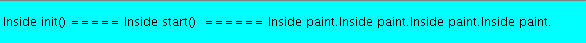
\includegraphics[width=\linewidth]{img_applet_1.jpg}
  \label{fig:boat1}
\end{figure}


\textbf{Problem 8.2} \textit{ Write a program to draw various shapes in an applet using Applet class.}

\textit{Code.}

\begin{lstlisting}
import java.awt.*;
import java.applet.*;
public class a extends Applet
{
	String msg="";
	int posx=25;
	int posy=25;
	public void init()
	{
		setForeground(Color.red);
		setBackground(Color.cyan);
		msg+="Inside init() ===== ";
	}
	public void start()
	{
		msg+="Inside start()  ====== ";
	}
	public void paint(Graphics g)
	{
		msg+="Inside paint.";
		g.drawString(msg, posx, posy);
		setForeground(Color.red);
		int x[]={10,20,10};
		int y[]={10,20,30};
		g.drawPolygon(x, y, 3);
		int x1[]={60,100,60,100};
		int y1[]={60,60,100,100};
		g.fillPolygon(x1,y1,4);
		g.drawOval(150,150,50,100);
		g.fillOval(200,200,50,50);
		int x2[]={100,200};
		int y2[]={100,100};
		g.drawPolygon(x2,y2,2);
		g.drawRect(200,100,60,60);
		g.fillRect(80,100,60,60);
	}
	public void stop()
	{}
	public void destroy()
	{}
}
\end{lstlisting}

\textit{Output.}

\begin{figure}[h!]
  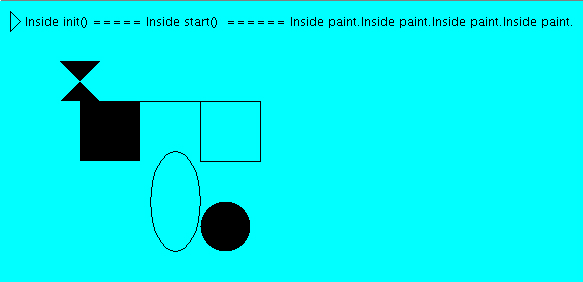
\includegraphics[width=148mm]{img_applet_2.jpg}
  \label{fig:boat1}
\end{figure}


\section{Week 9 - Exception Handling}
\textbf{Problem 9.1} \textit{Demonstrate the use of try\{..\} finally\{...\} block}

\textit{Code.}
\begin{lstlisting}
import java.util.*;
import java.lang.*;
import java.io.*;
class Exep
{
	public static void main (String[] args)
	{
		int a[]={1,2,3,4,5};
		try {
		    System.out.println(a[5]);
		} finally {
		    System.out.println("Finally executed");
		}
	}
}
\end{lstlisting}

\textit{Output.}
\begin{lstlisting}
Finally executed
Exception in thread "main" java.lang.ArrayIndexOutOfBoundsException: 5
	at Exep.main(Main.java:10)
\end{lstlisting}

\textbf{Problem 9.2} \textit{Demonstrate the use of try\{..\} catch\{...\} finally\{...\} block}

\textit{Code.}
\begin{lstlisting}
import java.util.*;
import java.lang.*;
import java.io.*;
class Exep2
{
	public static void main (String[] args)
	{
		int a[]={1,2,3,4,5};
		try {
		    System.out.println(a[5]);
		} catch(Exception e) {
		    System.out.println("Error: "+e);
		} finally {
		    System.out.println("Finally executed");
		}
	}
}
\end{lstlisting}

\textit{Output.}
\begin{lstlisting}
Error: java.lang.ArrayIndexOutOfBoundsException: 5
Finally executed
\end{lstlisting}

\textbf{Problem 9.3} \textit{Demonstrate the use of try\{..\} catch(Exception e1)\{...\} catch(Exception e2)\{...\} finally\{...\} block}

\textit{Code.}
\begin{lstlisting}
import java.util.*;
import java.lang.*;
import java.io.*;
class Exep3
{
	public static void main (String[] args)
	{
		int a[]={1,2,3,4,5};
		try {
		    System.out.println(a[5]);
		} catch(ArrayIndexOutOfBoundsException e) {
		    System.out.println("IndexOutOfBoundsException ");
		} catch(Exception e) {
		    System.out.println("Error: "+e);
		} finally {
		    System.out.println("Finally executed");
		}
	}
}
\end{lstlisting}

\textbf{Problem 9.4} \textit{Demonstrate the use of User defined exceptions using the Bank Problem}

\textit{Code.}
\begin{lstlisting}
import java.util.*;
class myException extends Exception
{
	public void show()
	{
		System.out.println("Not enough Balance");
	}
}
class Bank{
	static Scanner sc=new Scanner(System.in);
	static long acno; static double amt;
	static String id;
	private void init(){
		acno=0; amt=0.0;
		id="";
	}
	private double deposit(double d){ return amt+=d; }
	private double withdraw(double d){
		if(d<amt&&amt!=0)return amt-=d;
		else {
			try {
				throw new myException();
			} catch(myException e)
			{
				e.show();
			}
		}
		return -1;
	}
	private void print(){
		System.out.println("Customer ID \t A/c No. \t"+
		"Current Balance");
		System.out.println(id+"\t \t "+acno+"\t \t "+amt);
	}
	public static void main(String[]args){
		Bank obj=new Bank();
		obj.init();
		System.out.println("Enter account no and current balance:");
		id="3000114022";
		acno=sc.nextLong(); amt=sc.nextDouble();
		double d=0.0;
		int choice=0;
		do{
			System.out.println("Main Menu");
			System.out.println("0. Deposit");
			System.out.println("1. Withdrawal");
			System.out.println("2. Print Statement");
			System.out.println("3. Exit");
			System.out.println("Enter choice:");
			choice=sc.nextInt();
			switch(choice){
				case 0:d=0.0;
				        System.out.println("Enter "+
				        "amount to deposit:");
				        d=sc.nextDouble();
					 System.out.println("Deposit="+d+
					 "current balance="+
					 (double)obj.deposit(d));
					 break;
				case 1:d=0.0;
				       System.out.println("Amount ?");
				       d=sc.nextDouble();
				       System.out.println("withdrawal="+d+
				       "current balance="+
				       (double)obj.withdraw(d));
				        break;
				case 2:obj.print();
				       break;
				default:
					break;
			}
		}while(choice<3);
	}
}
\end{lstlisting}

\textit{Output.}
\begin{lstlisting}
Enter account no and current balance:
100
200
Main Menu
0. Deposit
1. Withdrawal
2. Print Statement
3. Exit
Enter choice:
1
Amount ?
5000
Not enough Balance
withdrawal=5000.0current balance=-1.0
Main Menu
0. Deposit
1. Withdrawal
2. Print Statement
3. Exit
Enter choice:
3
\end{lstlisting}

%\begin{theorem}
%This is a theorem statement.
%\label{thm:sample-statement}
%\end{theorem}

%\proof{
%This is a proof.
%}



\end{document}
\grid
